\subsection{Procesamiento}

Se tomaron en cuenta especificaciones sobre el brazo robótico a controlar y los servomotores posicionales a los que se envían las instrucciones.

El tipo de brazo robótico a controlar tiene un diseño antropomórfico, lo que significa que se compone de eslabones unidos por articulaciones entre sí; además es de dos grados de libertad, lo que implica que tiene exactamente dos articulaciones. Como lo que interesa es controlar la posición (y no la orientación), se restringió la cantidad de grados de libertad del brazo robótico a uno en cada articulación; esto significa que en la unión entre la base y el primer eslabón existe un grado de libertad, y el otro grado de libertad se encuentra en la unión entre el primer y segundo eslabón. Además, ambas articulaciones rotan en un plano perpendicular al eje horizontal del robot. Para alcanzar todas las posiciones posibles en el espacio, existe un grado de libertad adicional en la base que rota el brazo robótico alrededor de su eje vertical. La Figura \ref{fig:tipobrazo} muestra un ejemplo de un brazo robótico que cumple con estas especificaciones.

\begin{figure}[htb]
	\centering
	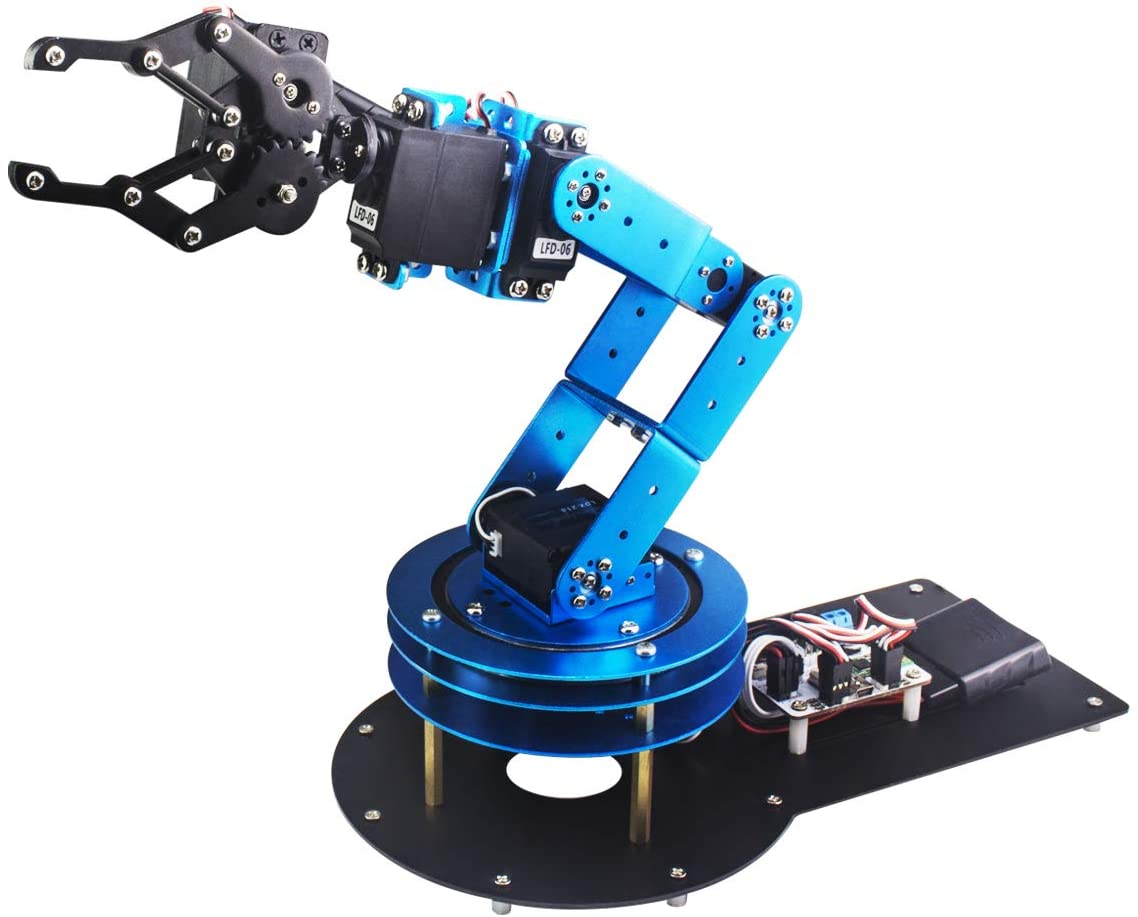
\includegraphics[scale=0.15]{tipobrazo.jpg}
	\caption{Brazo robótico de 2 DoF que cumple las restricciones impuestas}
	\label{fig:tipobrazo}
\end{figure}

El brazo robótico tiene la base en el suelo; esto significa que se puede mover dentro y en el contorno curvo de la mitad de una esfera con centro en la base del robot y de radio igual a la longitud del robot; debido a que la ortesis utilizada para localizar la posición tiene 42 cm de largo, ésta es la máxima longitud del brazo para el sistema. Los servomotores posicionales solo pueden moverse en ángulos discretos. Esto significa que pueden alcanzar 180 posiciones. Además, muchas posiciones finales son lo suficientemente cercanas entre sí como para considerar que se aproximan a la misma posición.  Para determinar la proximidad de las posiciones, se aplicó el siguiente criterio con distancia Euclidiana entre dos posiciones. Si $P_1 = (x_1, y_1, z_1)$ es un punto en el espacio tal que sus coordenadas son valores enteros y $P_2 = (x_2, y_2, z_2)$ es cualquier otro punto:

\begin{equation}
	d(P_1, P_2) = |\sqrt{(x_2 - x_1)^2 + (y_2 - y_1)^2 + (z_2 - z_1)^2} <= \approx 0,65 cm
\end{equation}

Donde la cota establecida es la máxima distancia euclidiana obtenida; esta es la distancia de un punto $P_1$ al centro de un cubo de 1 cm donde $P_1$ es un vértice del cubo; de este modo, se considera que aquellos puntos que tienen a lo más 0,65 cm de distancia euclidiana entre ellos llegan a la misma posición. Para el caso en el que una de las coordenadas del punto $P_2$ sea entera, su distancia euclidiana al punto $P_1$ más cercano será menor que o igual a 0,5 cm. Si las posiciones alcanzables son como el punto $P_1$ antes descrito, esto significa que es posible agrupar ciertas poses para alcanzar una determinada región muy pequeña en el espacio.

Se consideró que los servomotores son colocados inicialmente paralelos al eje horizontal. Podemos notar que muchas posiciones pueden ser alcanzadas por un brazo robótico de una determinada longitud de articulaciones con más de una combinación de ángulos; por ejemplo, si la base tiene 0°, y ambas articulaciones tienen 90° y 0°, respectivamente, se alcanza la misma posición que si la base tiene 180°, y ambas articulaciones tienen 90° y 180°, respectivamente. En particular, si colocamos un plano paralelo al diámetro de la semiesfera que la atraviese, podemos notar las configuraciones ``espejo'' que alcanzan la misma posición. De modo que se restringió el rango de movilidad de las articulaciones de 0 a 90°; la base se mantuvo de 0 a 360°. 

%Si consideramos además que las longitudes de los brazos varían, esto significa que cada punto $P_1$ puede ser alcanzado por varias combinaciones distintas de longitudes de articulaciones y ángulos. Esto se aprovechó para reducir la cantidad de operaciones realizadas para determinar la cinemática inversa; dada una posición $P = (x,y,z)$ con las características de $P_1$, existe un conjunto de combinaciones de longitudes de articulaciones y ángulos de inclinación que alcanzan dicha posición (aplicando el criterio de la distancia euclidiana). Se consideró que estaban asociadas a dicha posición.

Esto nos da las siguientes restricciones para generar el conjunto de datos:

\begin{itemize} 
	
	\item $\alpha_1, \alpha_2, \alpha_3 \in \mathbb{Z}$; El ángulo de la base es $ 0 \leq \alpha_1 \leq 360$, mientras que los ángulos de inclinación de las articulaciones son $ 0 \leq \alpha_2, \alpha_3 \leq 90$
	
	\item Las posiciones alcanzables $P = (x, y, z)$ son tales que $x,y,z \in \mathbb{Z}$, y se asocian con un conjunto de ángulos $\alpha_1, \alpha_2, \alpha_3$ que, al ser aplicados para obtener una posición final $P_f(x_f,y_f,z_f)$, sea el punto con menor distancia euclidiana al punto $P$. La posición $P_f$ se calcula con las siguientes ecuaciones, derivada de la matriz de rotacion de la especificación mencionada del brazo robótico:
	
\end{itemize}

%\begin{equation}
%	x = L_1 \cdot \cos(\alpha_2) \cdot \cos(\alpha_1) + L_2 \cdot \cos(\alpha_2 + \alpha_3) \cdot \cos(\alpha_1)
%\end{equation}

%\begin{equation}
%	y = L_1 \cdot \cos(\alpha_2) \cdot \sin(\alpha_1) + L_2 \cdot \cos(\alpha_2 + \alpha_3) \cdot \sin(\alpha_1)
%\end{equation}

%\begin{equation}
%	z = L_1 \cdot \sin(\alpha_2) + L_2 \cdot \sin(\alpha_2 + \alpha_3) \cdot \cos(\alpha_1)
%\end{equation}

\begin{equation}
	x = L_1 \cos(\alpha_1) \cdot \cos(\alpha_3) + L_2 \cos(\alpha_1 + \alpha_2) \cdot \cos(\alpha_3)
\end{equation}

\begin{equation}
	y = L_1 \cos(\alpha_1) \cdot \sin(\alpha_3) + L_2 \cos(\alpha_1 + \alpha_2) \cdot \sin(\alpha_3)
\end{equation}

\begin{equation}
	z = L_1 \sin(\alpha_1) + L_2 \sin(\alpha_1 + \alpha_2)
\end{equation}

Los ángulos con las restricciones anteriores se almacenaron en archivos binarios de acuerdo con la posicion especifica. De este modo, cuando se ingrese una posición $P(x,y,z)$ con longitudes $L_1, L_2$, primero, se determina el punto más cercano $P_i(x_i,y_i,z_i)$ a $P(x,y,z)$ tal que $x_i,y_i,z_i \in \mathbb{Z}$ de los 8 puntos que rodean a $P(x,y,z)$, si se considera esta posición dentro de un cubo (las esquinas $P_i(x_i,y_i,z_i)$ son parte de los puntos como $P_1$ revisados antes); posteriormente, se busca el archivo binario que se corresponde con dicha posición; si no existe, quiere decir que el brazo no puede llegar a dicha posición. De lo contrario, la combinación de ángulos $\alpha_1, \alpha_2, \alpha_3$ guardados en el archivo binario se toma como la salida de la etapa de Procesamiento.